%% Semplice beamer conforme al powerpoint ufficiale
%% dal sito di Ca' Foscari. Si basa sul tema "default"
%% mandate Modifiche e migliorie! Guido.Caldarelli@unive.it 
% Elenco Contributori 
% Guido Caldarelli, Matteo Brilli 

%\documentclass{beamer}
% decide below the aspect ratio between 16:9 and 4:3
%\documentclass[aspectratio=43]{beamer}
\documentclass[aspectratio=169]{beamer}

\usepackage[utf8]{inputenc}
\usepackage{tikz}
\usepackage{multicol}
% Questo tema commentato di sotto produce un beamer più tradizionale 
%\usetheme[secheader]{Boadilla}


%%%-----------------------------------------------------------%
%% Cambia colori da thema default
%% Questi sono i due colori ufficiali rosso e grigio
\definecolor {cfred}{rgb}{0.709,0.196,0.329} 	%{ 181 ,50 ,84}
\definecolor {cfgrey}{rgb}{0.537,0.537,0.537} 	%{ 137,137,137}
\definecolor {cflink}{rgb}{0.615,0.615,0.607} 	%{157,157,155}

\setbeamercolor{palette primary}{bg=cfred,fg=white}
\setbeamercolor{palette secondary}{bg=cfred,fg=white}
\setbeamercolor{palette tertiary}{bg=cfred,fg=white}
\setbeamercolor{palette quaternary}{bg=cfred,fg=white}
\setbeamercolor{structure}{fg=cfred}		 % itemize, enumerate, etc
\setbeamercolor{section in toc}{fg=cfred} 		 % TOC sections
% Override palette coloring with secondary
\setbeamercolor{subsection in head/foot}{bg=cfgrey,fg=white}
%%%------------------------------------------------------------

%% Definisce il blocco con riquadro che non è presente nel tema default (commentare se si usano altri temi)
\setbeamercolor{uppercolor}{fg=white,bg=cfred}%
\setbeamercolor{lowercolor}{fg=black,bg=white}%
\def \bblock{\begin{beamerboxesrounded}[upper=uppercolor,lower=lowercolor,shadow=true]}
\def \eblock{\end{beamerboxesrounded}}
%%-----------------------------------------------------------
\setbeamertemplate{footline}[frame number]
\setbeamertemplate{caption}{\raggedright\insertcaption\par}
%% Intestazione ripetuta per ogni slide
\addtobeamertemplate{headline}{%
\vspace{0.25cm} \ \ 

\includegraphics[height=1.0cm]{kicc.png} 	% sostituire con logobeamIT.png per italiano
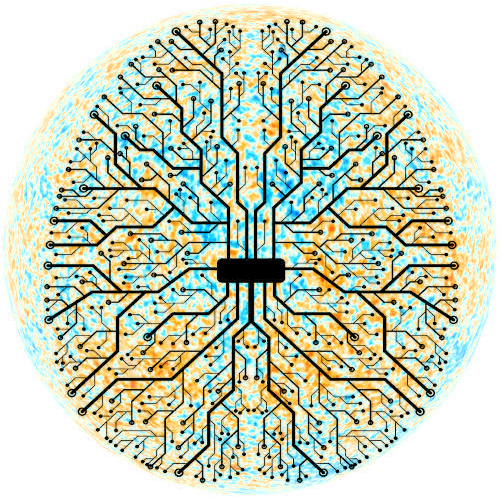
\includegraphics[height=1.0cm]{Ca_Foscari Beamer/handley-lab.png}
%\hspace{0.641\textwidth}{\color{cflink} {\small www.unive.it}} %per 16:9
%\hspace{0.551\textwidth}{\color{cflink} {\small www.unive.it}} %per 4::3

\vspace{0.25cm}
{\color{cfred} \hrule \hrule  }
\textbf{}
}{}
%%-------------------------------------------------------------

%This block of code defines the information to appear in the Title page
%%%
\title[Accelerated nested sampling with $\beta$-flows] %optional
{Accelerated nested sampling with $\beta$-flows}

\author[Metha Prathaban] % (optional)
{Metha Prathaban \break myp23@cam.ac.uk}




\setbeamertemplate{frametitle}[default][right, rightskip=.5cm] {}
\addtobeamertemplate{frametitle}{\vspace*{-1.4cm}}{}
%End of title page configuration block
%------------------------------------------------------------


%------------------------------------------------------------
%The next block of commands puts the table of contents at the 
%beginning of each section and highlights the current section:

% \AtBeginSection[]
% {
%   \begin{frame}
%     \frametitle{Table of Contents}
%     \tableofcontents[currentsection]
%   \end{frame}
% }
%------------------------------------------------------------

\begin{document}

%The next statement creates the title page.
\frame{\titlepage}
%---------------------------------------------------------
%This block of code is for the table of contents after
%the title page
\begin{frame}
\frametitle{About Me}
\begin{itemize}
    \item 3rd year PhD student in Will Handley's group
    \item Work on gravitational waves and Bayesian numerical method development
    \item Office in K34
\end{itemize} 
\vspace{2em}
\bblock{\begin{center}
The Handley group!
\end{center}}
\begin{center}
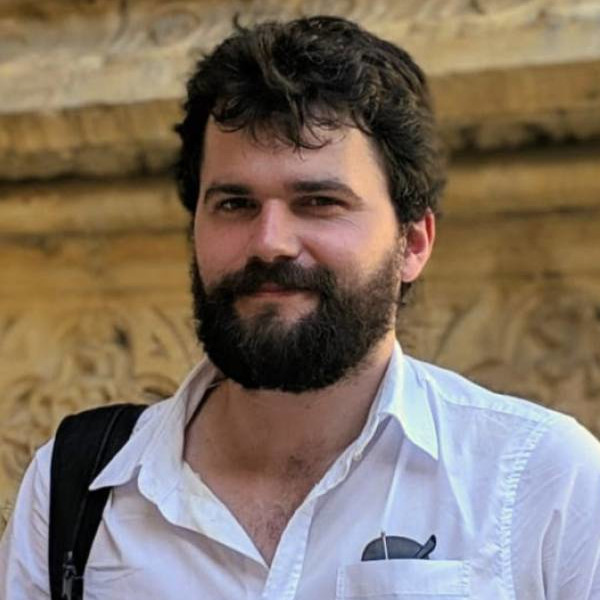
\includegraphics[height=1.0cm]{Ca_Foscari Beamer/will_handley.jpg}
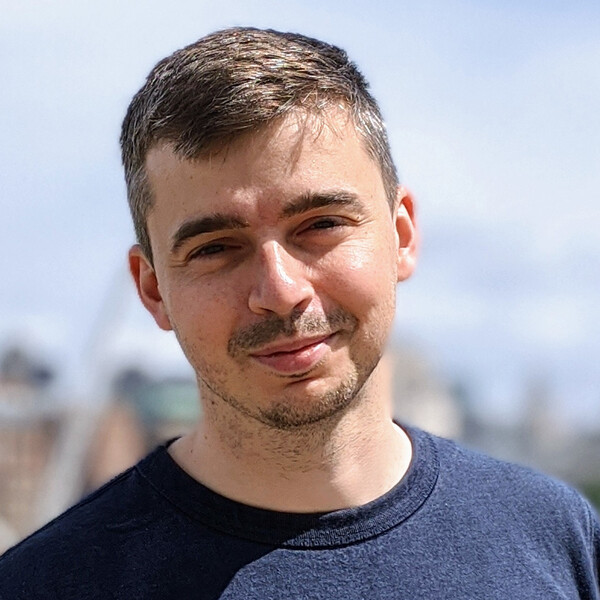
\includegraphics[height=1.0cm]{Ca_Foscari Beamer/david_yallup.jpg}

\includegraphics[height=1.0cm]{Ca_Foscari Beamer/harry_bevins.jpg}

\includegraphics[height=1.0cm]{Ca_Foscari Beamer/adam_ormondroyd.jpg}
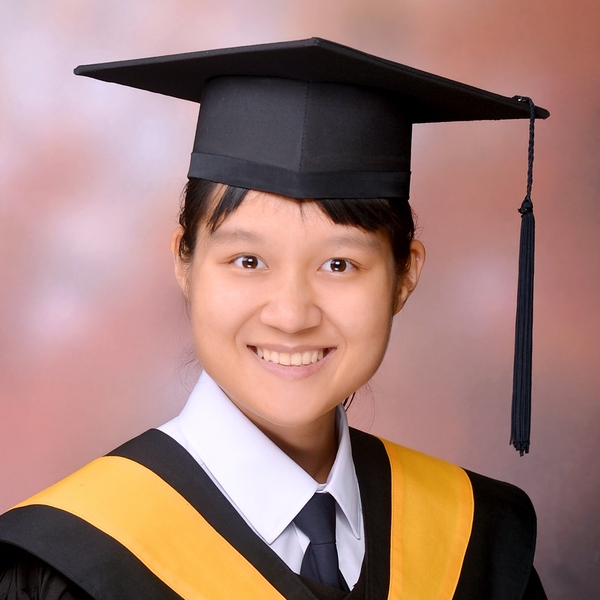
\includegraphics[height=1.0cm]{Ca_Foscari Beamer/wei-ning_deng.jpg}

\includegraphics[height=1.0cm]{Ca_Foscari Beamer/metha_prathaban.jpg}
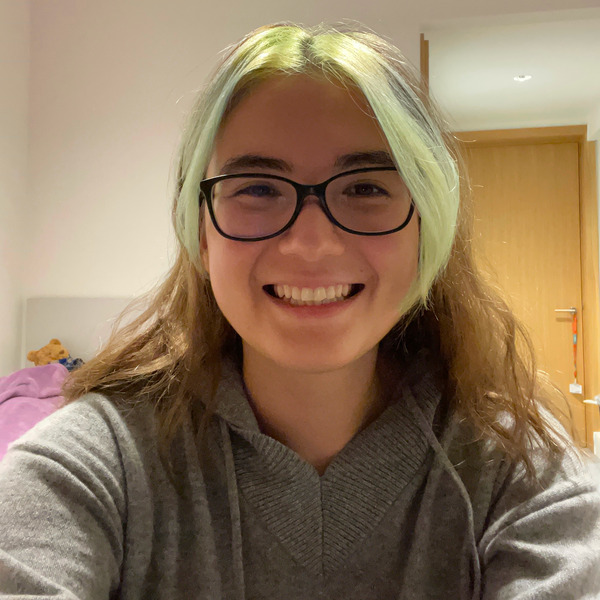
\includegraphics[height=1.0cm]{Ca_Foscari Beamer/sinah_legner.jpg}
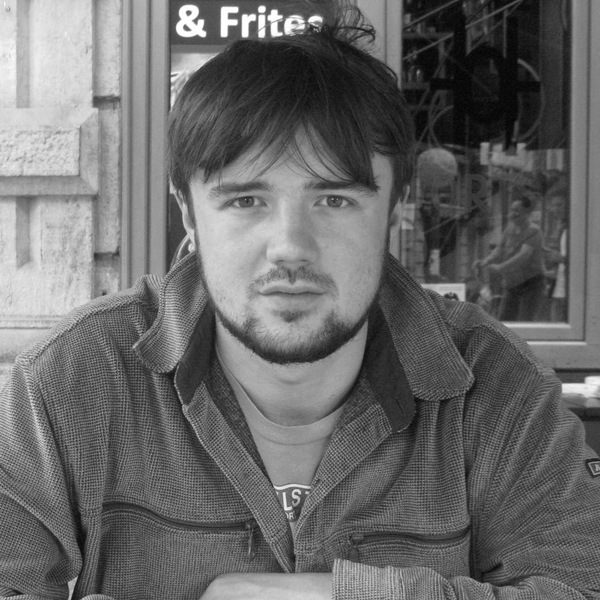
\includegraphics[height=1.0cm]{Ca_Foscari Beamer/sam_leeney.jpg}
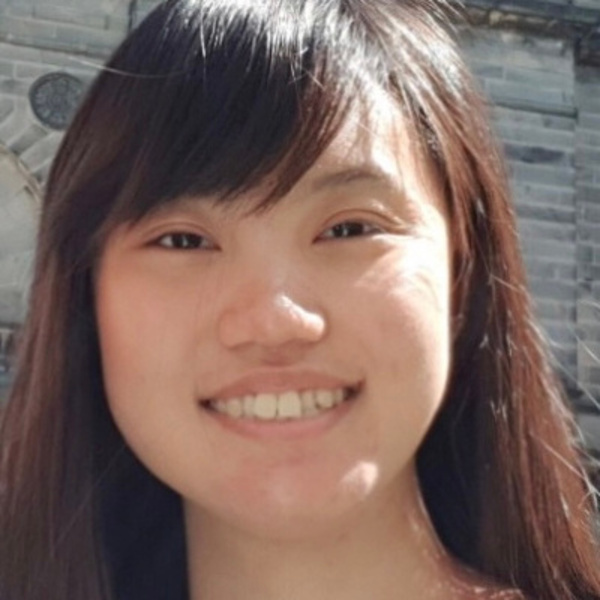
\includegraphics[height=1.0cm]{Ca_Foscari Beamer/dily_ong.jpg}

\includegraphics[height=1.0cm]{Ca_Foscari Beamer/namu_kroupa.jpg}
\end{center}
\begin{center}
    + Part III students + others!
\end{center}
\eblock
\end{frame}


%This block of code is for the table of contents after
%the title page
\begin{frame}
\frametitle{Table of Contents}\vspace{2em}
\bblock{\begin{center}
Current work is in collaboration with Will Handley and Harry Bevins.
\end{center}}
\begin{center}
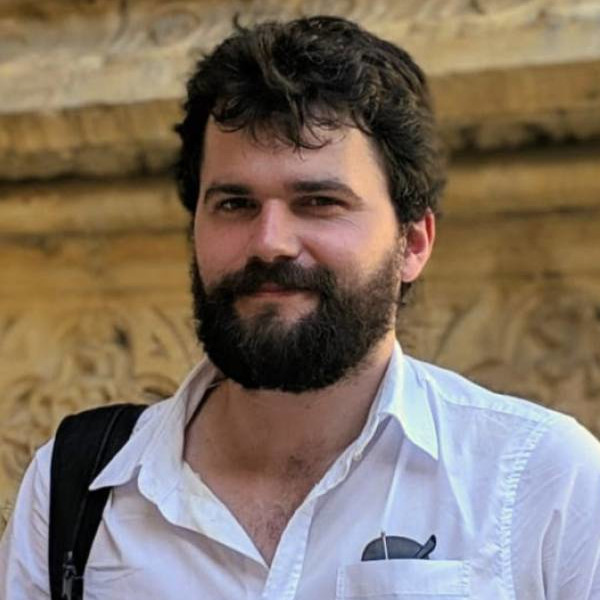
\includegraphics[height=2.0cm]{Ca_Foscari Beamer/will_handley.jpg}

\includegraphics[height=2.0cm]{Ca_Foscari Beamer/harry_bevins.jpg}
\end{center}
\eblock
\tableofcontents
\end{frame}
%---------------------------------------------------------


%\section{Nested sampling}


%---------------------------------------------------------
%Changing visibility of the text
\begin{frame}
\frametitle{Bayes' Theorem for Gravitational Waves}
\begin{minipage}{\textwidth}\vspace{1em}
    Given some model $\mathcal{M}$ and observed signal $\mathcal{D}$, Bayes' theorem enables us to relate the posterior probability of the set of parameters $\theta$ which generated the signal to the likelihood of the $\mathcal{D}$ given $\theta$ and the prior probability of $\theta$ given $\mathcal{M}$:
\end{minipage}
\begin{minipage}{0.22\textwidth}\vspace{0.5em}
\begin{figure}
\centering
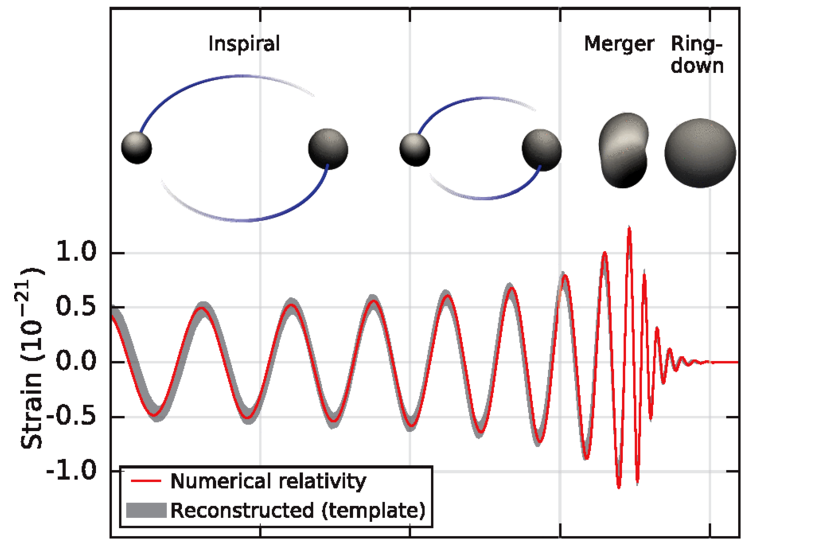
\includegraphics[height=0.95\textwidth]{Ca_Foscari Beamer/Screenshot from 2024-10-14 13-25-30.png}
\caption{\textcolor{cfgrey}{Abbott et al. arXiv:1602.03837}}
\end{figure}
\end{minipage}
\hspace{30pt}
\begin{minipage}{0.6\textwidth}
\centering
\begin{align*}
    P(\theta | D, \mathcal{M}) = \frac{P(D | \theta, \mathcal{M}) P(\theta | \mathcal{M})}{P(D | \mathcal{M})} = \frac{\mathcal{L}(D | \theta)\pi(\theta)}{\mathcal{Z}}
\end{align*}
\end{minipage}%
\vfill
\begin{minipage}{\textwidth}
The evidence, $\mathcal{Z}$, plays a key role in model comparison.
\end{minipage}
\end{frame}

%---------------------------------------------------------


%---------------------------------------------------------
%Example of the \pause command
\begin{frame}
\frametitle{Nested sampling (NS)}
\begin{minipage}[]{0.3\textwidth}
\vspace{20em}
\begin{tikzpicture}
\def\svgwidth{\textwidth}
\input{schematic_revised_latex_big.pdf_tex}
\end{tikzpicture}
\textcolor{cfgrey}{2404.16428}
\end{minipage}\hfill
\begin{minipage}{0.6\textwidth}
    \begin{itemize}
        \item<1-> Nested sampling first and foremost calculates the evidence (\textsc{MultiNest} \textcolor{cfgrey}{0809.3437}, \textsc{dynesty} \textcolor{cfgrey}{1904.02180}, \textsc{nessai} \textcolor{cfgrey}{2102.11056} and \textsc{PolyChord} \textcolor{cfgrey}{1506.00171})
        \item<2-> Prior is populated with set of `live points'.
        \item<3-> At each iteration $i$, point with lowest likelihood is deleted and new live point is drawn, which must have a \textbf{likelihood higher than that of the deleted point.}
        \item<4-> Evidence is calculated as weighted sum over deleted (`dead') points.
    \end{itemize}
    \vspace{-2.5em}
\end{minipage}
\end{frame}
%---------------------------------------------------------

%\section{Accelerated NS}

%---------------------------------------------------------

\begin{frame}{Accelerating NS}

\begin{block}{Time of convergence of NS}
    \begin{equation}
        T \propto n_{\textrm{live}} \times T_{\mathcal{L}} \times f_{\textrm{sampler}} \times D_{\textrm{KL}}
    \end{equation}
\end{block}

\begin{block}{Uncertainty in log$\mathcal{Z}$}
    \begin{equation}
        \sigma \propto \sqrt{D_{\textrm{KL}} / n_{\textrm{live}}}
    \end{equation}
\end{block}

\alert{Precision-normalized} runtime has quadratic dependence on KL divergence -- want to reduce amount of compression from prior to posterior. \textcolor{cfgrey}{Petrosyan \& Handley 212.01760}
    
\end{frame}

\begin{frame}{Reducing $D_{\textrm{KL}}$}

\begin{itemize}
    \item<1-> REACH collaboration do this already (see e.g. \textcolor{cfgrey}{Anstey et al. 2010.09644}):
        \begin{itemize}
            \item Perform a low-res pass of NS
            \item Identify rough region of posterior and set box prior around this
            \item Full high-res run with narrower prior
            \item Need to correct the evidence as the prior has changed. 
        \end{itemize}

    \item<2-> Can use \textbf{machine learning} to learn the rough posterior distribution from pass 1, and use as proposal for pass 2. 

    \item<3-> \alert{Posterior repartitioning (PR)} (\textcolor{cfgrey}{Chen et al. 1803.06387 \& 1908.04655}) allows one to do this \textbf{without needing to correct evidence} (see e.g. \textcolor{cfgrey}{Petrosyan \& Handley 2212.0176}).

\end{itemize}
\end{frame}

%\section{$\beta$-flows}

\begin{frame}{$\beta$-flows vs typical NFs}
    \begin{minipage}[]{0.35\textwidth}
    \vspace{3em}
    \begin{figure}
        \centering
        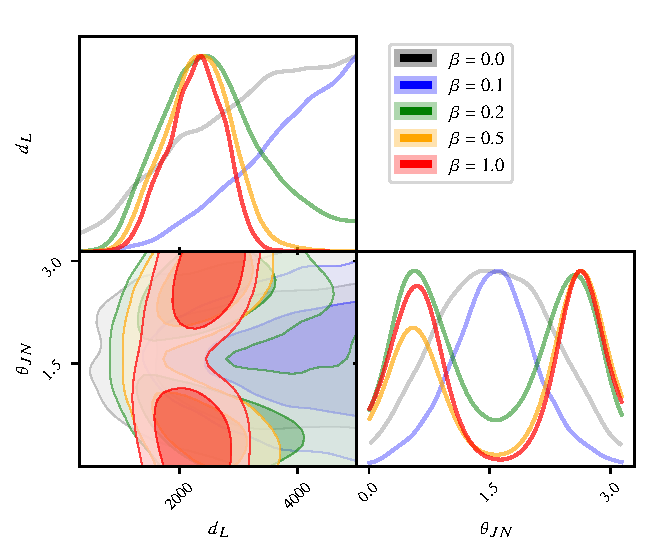
\includegraphics[width=\textwidth]{Ca_Foscari Beamer/temperature_comparison.pdf}
        %\caption{Caption}
        %\label{fig:enter-label}
    \end{figure}
    \end{minipage}\hfill
    \begin{minipage}[]{0.6\textwidth}
    \begin{itemize}
    \item NFs can perform density estimation of posteriors from NS/other sampling method. 
    \item Nested sampling gives you a lot more information than just the posterior samples - we have access to samples at every ``temperature''. 
    \item In statistical mechanics, this temperature is used in context of partition function.
    \item Idea of $\beta$-flows is to explore this arm of NS to learn posterior better. 
    %\item Bonus: $\beta$-flows learn all the intermediate stages from prior to posterior, so can choose a ``wider" proposal for high-res pass if we want.
    \end{itemize}
    \end{minipage}
\end{frame}

\begin{frame}{}
\centering
    Thank you for listening!
\end{frame}

%Highlighting text
\begin{frame}{Posterior repartitioning (PR)}
Unlike other sampling algorithms, such as Metropolis-Hastings or Hamiltonian Monte Carlo, NS distinguishes between $\mathcal{L}$ and $\pi$ by \alert{`sampling from the prior, subject to the hard likelihood constraint, $\mathcal{L}$'}.

But evidence and posteriors only depend on product of $\mathcal{L}$ and $\pi$: \vspace{-2em}
\begin{multicols}{2}
\begin{equation}
    \mathcal{Z} = \int \mathcal{L}(\theta) \pi(\theta) d\theta
\end{equation}\break
\begin{equation}
    \mathcal{P}(\theta) = \frac{\mathcal{L}(\theta)\pi(\theta)}{\mathcal{Z}}
\end{equation}
\end{multicols}
\bblock{Therefore, we are free to redefine the likelihood and prior however we like - as long as the product is the same! \textcolor{cfgrey}{arXiv:1908.04655}}
    \centering
    \begin{equation}
        \tilde{\mathcal{Z}} = \int \tilde{\mathcal{L}}(\theta) \tilde{\pi}(\theta) d\theta = \int \mathcal{L}(\theta) \pi(\theta) d\theta = \mathcal{Z}
    \end{equation}
\eblock
\end{frame}

% \begin{frame}{Normalizing flows as posterior density estimators}
% \begin{minipage}{0.45\textwidth}\vfill
%         \begin{figure}
%         \centering
%         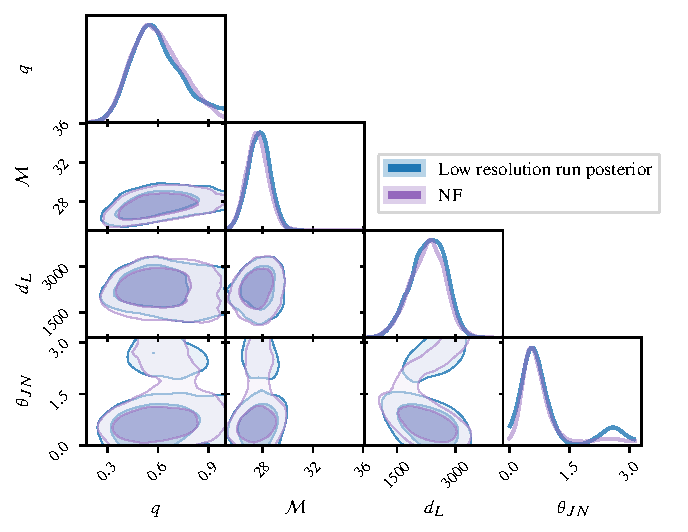
\includegraphics[width=0.9\textwidth]{Ca_Foscari Beamer/15param_lowres_vs_nf.pdf}
%     \end{figure}
% \end{minipage}
% \begin{minipage}{0.45\textwidth}\vfill
%         \begin{figure}
%         \centering
%         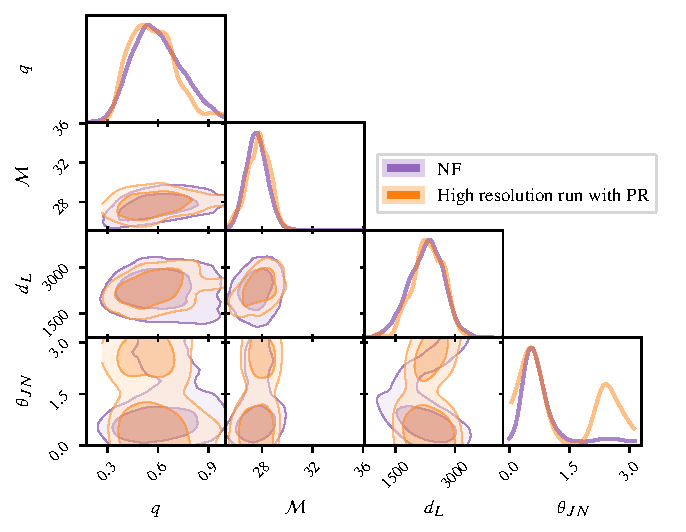
\includegraphics[width=0.9\textwidth]{Ca_Foscari Beamer/15param_highres_vs_nf.pdf}
%     \end{figure}
% \end{minipage}

% \vspace{2em}
% Same answer as doing a full resolution pass of NS, but \alert{6x faster}.

% \end{frame}

%---------------------------------------------------------

%---------------------------------------------------------


%---------------------------------------------------------

%---------------------------------------------------------


\end{document}